Goals: show we can work at scale ($S=1600$) of real public health problems, and do gradient learning effectively there. Still show how overcome misspecification to deliver good top-K predictions in this scaled up problem. Talk about specific hyperparameters in ALL experiments.

We also construct a dataset on the scale of real-world decision making problems in order to demonstrate the capabilities of decision-aware training on larger problems.

The data and results are described in Figure \ref{fig:synth_data2}. Here, the data exist on a 40-by-40 2D-grid ($S=1600$), approximately equivalent to the number of census tracts in Massachusetts. Here, the data consist of a large region of moderate values between $45^{\circ}$ and $90^{\circ}$. At $90^{\circ}$, the value is set to 14, and it gradually decreases to 9 at $45^\circ$. There also exists a narrow band of a large value (20) between $272^\circ$ and $280^\circ$. The entire grid then has a small amount of noise $\epsilon \sim \mathcal{N}(0, 0.5)$ added.  

To model the data, we again choose a misspecified model, as would exist in the real-world where we do not have knowledge of the true data generating process. Here, our model is:
\begin{align*}
    y_s &\sim \mathcal{N}(y_s|\mu_s, 0.2) \\
    \mu_s(\texttt{x},\texttt{y}) &= m \cdot  \exp\left(-\frac{d_{\perp}^2(\texttt{x},\texttt{y})}{2(l/10)^2}\right)
    \intertext{Where $\texttt{x}, \texttt{y}$ are the coordinates of the grid with the origin located in the middle and $d_{\perp}^2(\texttt{x},\texttt{y})$ is the perpendicular distance to the line:}
    \texttt{y} &= s \texttt{x}
\end{align*}

Our parameter vector $\phi$ then consists of 3 parameters: the magnitude $m$, the length scale $l$, and the slope of the line $s$. In order to find the best parameters, we perform a grid search over 10 magnitudes between 1 and 10, 20 lengthscales between 5 and 16, and 360 possible slopes between 0$^\circ$ and 359$^\circ$. We evaluate each hyperparameter setting with each objective: pure log likelihood, maximizing BPR-25, and a our hybrid objective in Eq. \ref{eq:hybrid_obj}.

\begin{figure}[!t]
\begin{center}
\begin{tabular}{c}
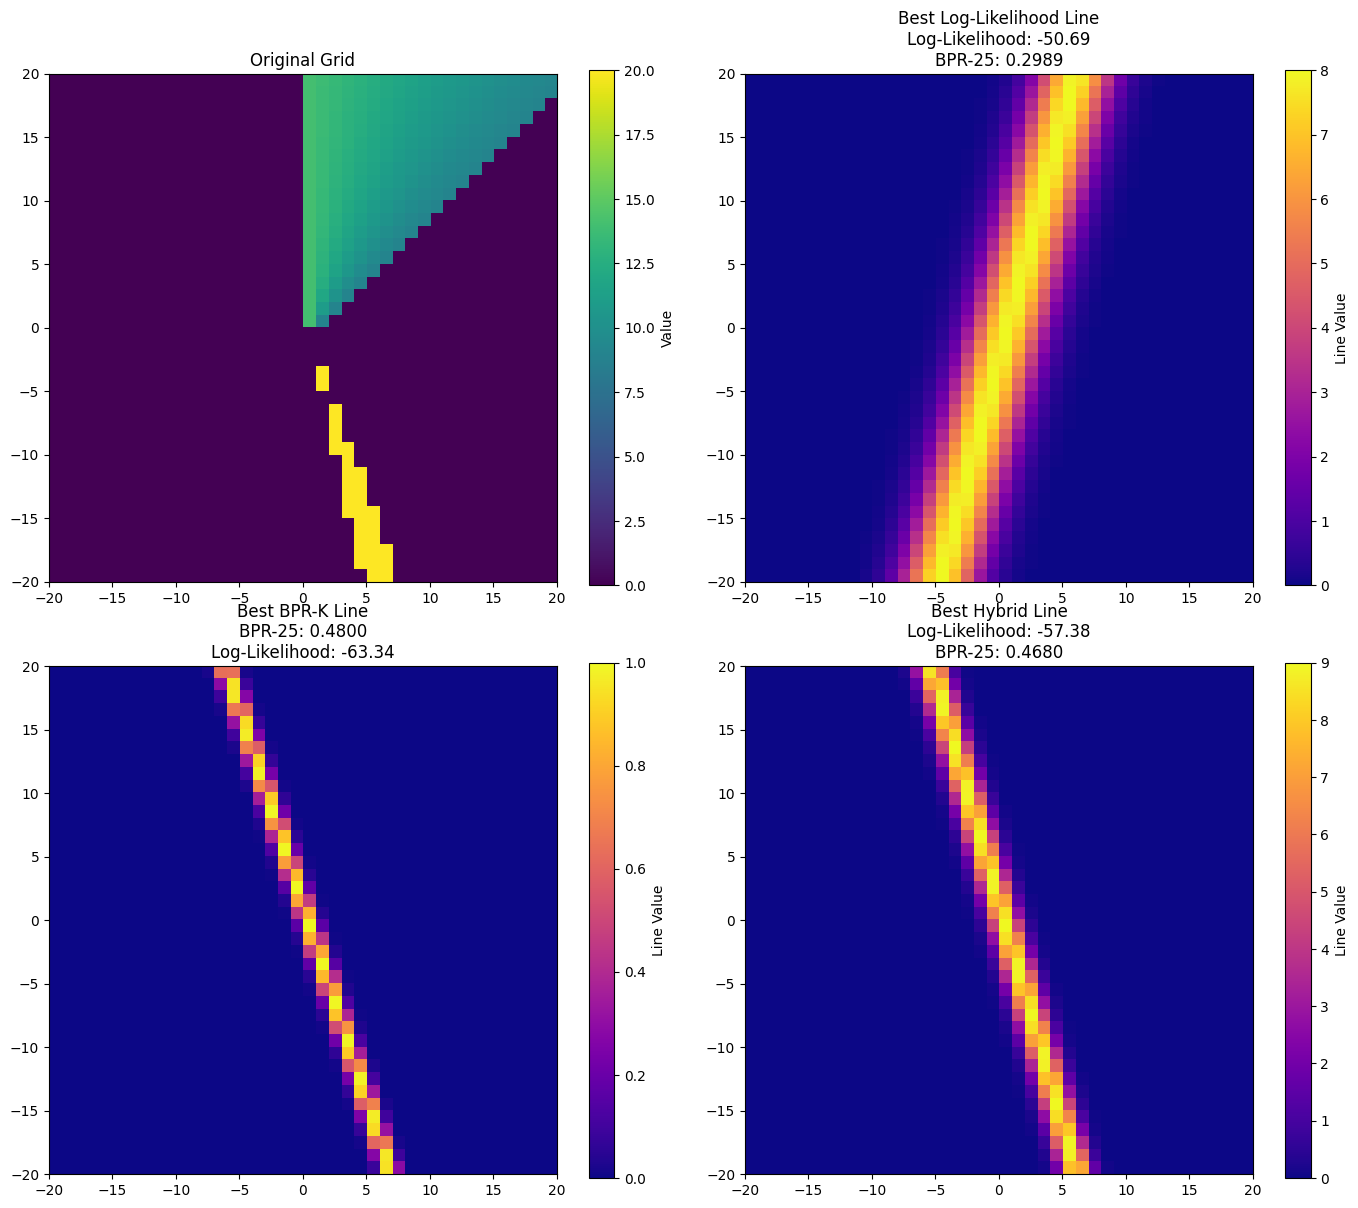
\includegraphics[width=.5\textwidth]{figures/synth_geo.png}
\end{tabular}
\end{center}
\captionof{figure}{
\textbf{Synthetic geospatial dataset and training results}. (Top left) The dataset for the synthetic geospatial training set. The data is on a 40-by-40 grid, which is roughly the number of Census tracts in Massachusetts. The data contains a large region of moderate values at the top, and a narrow band of high-valued locations at the bottom. When using a misspecified linear model, this results in the optimal ML and BPR solution being different 
(Top-right) The optimal ML solution. This model maximizes likelihood by capturing a large portion of the moderate-value region, but completely misses the high-value locations.
(Bottom-left) The optimal BPR solution is a narrow line which only captures the high-value locations. (Bottom-right) The optimal decision-aware solution also captures the high-valued locations.
}%end caption
\label{fig:synth_data2}
\end{figure}

The results are shown in Figure \ref{fig:synth_data2}. We see that in order to optimize log likelihood, we obtain a model with a large lengthscale covering the moderately-valued gradient, but models optimizing BPR-25 select the narrow, high-valued region. The hybrid objective can be tuned to select either case depending on choice of $\lambda$.
